\documentclass[12pt]{article}

\usepackage[spanish]{babel}
\usepackage[utf8]{inputenc}
\usepackage{graphicx}
\usepackage{geometry}
\usepackage{verbatim}
\usepackage{xcolor}
\usepackage{fancyhdr}
\usepackage{lastpage}
\usepackage{pdfpages}
\usepackage{listings}
\usepackage{schemata}

\geometry{top=25mm,left=15mm,right=15mm,a4paper}

\pagestyle{fancy}
\fancyhf{}
\lhead{Computación Concurrente}
\cfoot{Página \thepage\ de \pageref{LastPage}}

\graphicspath{./}

\begin{document}
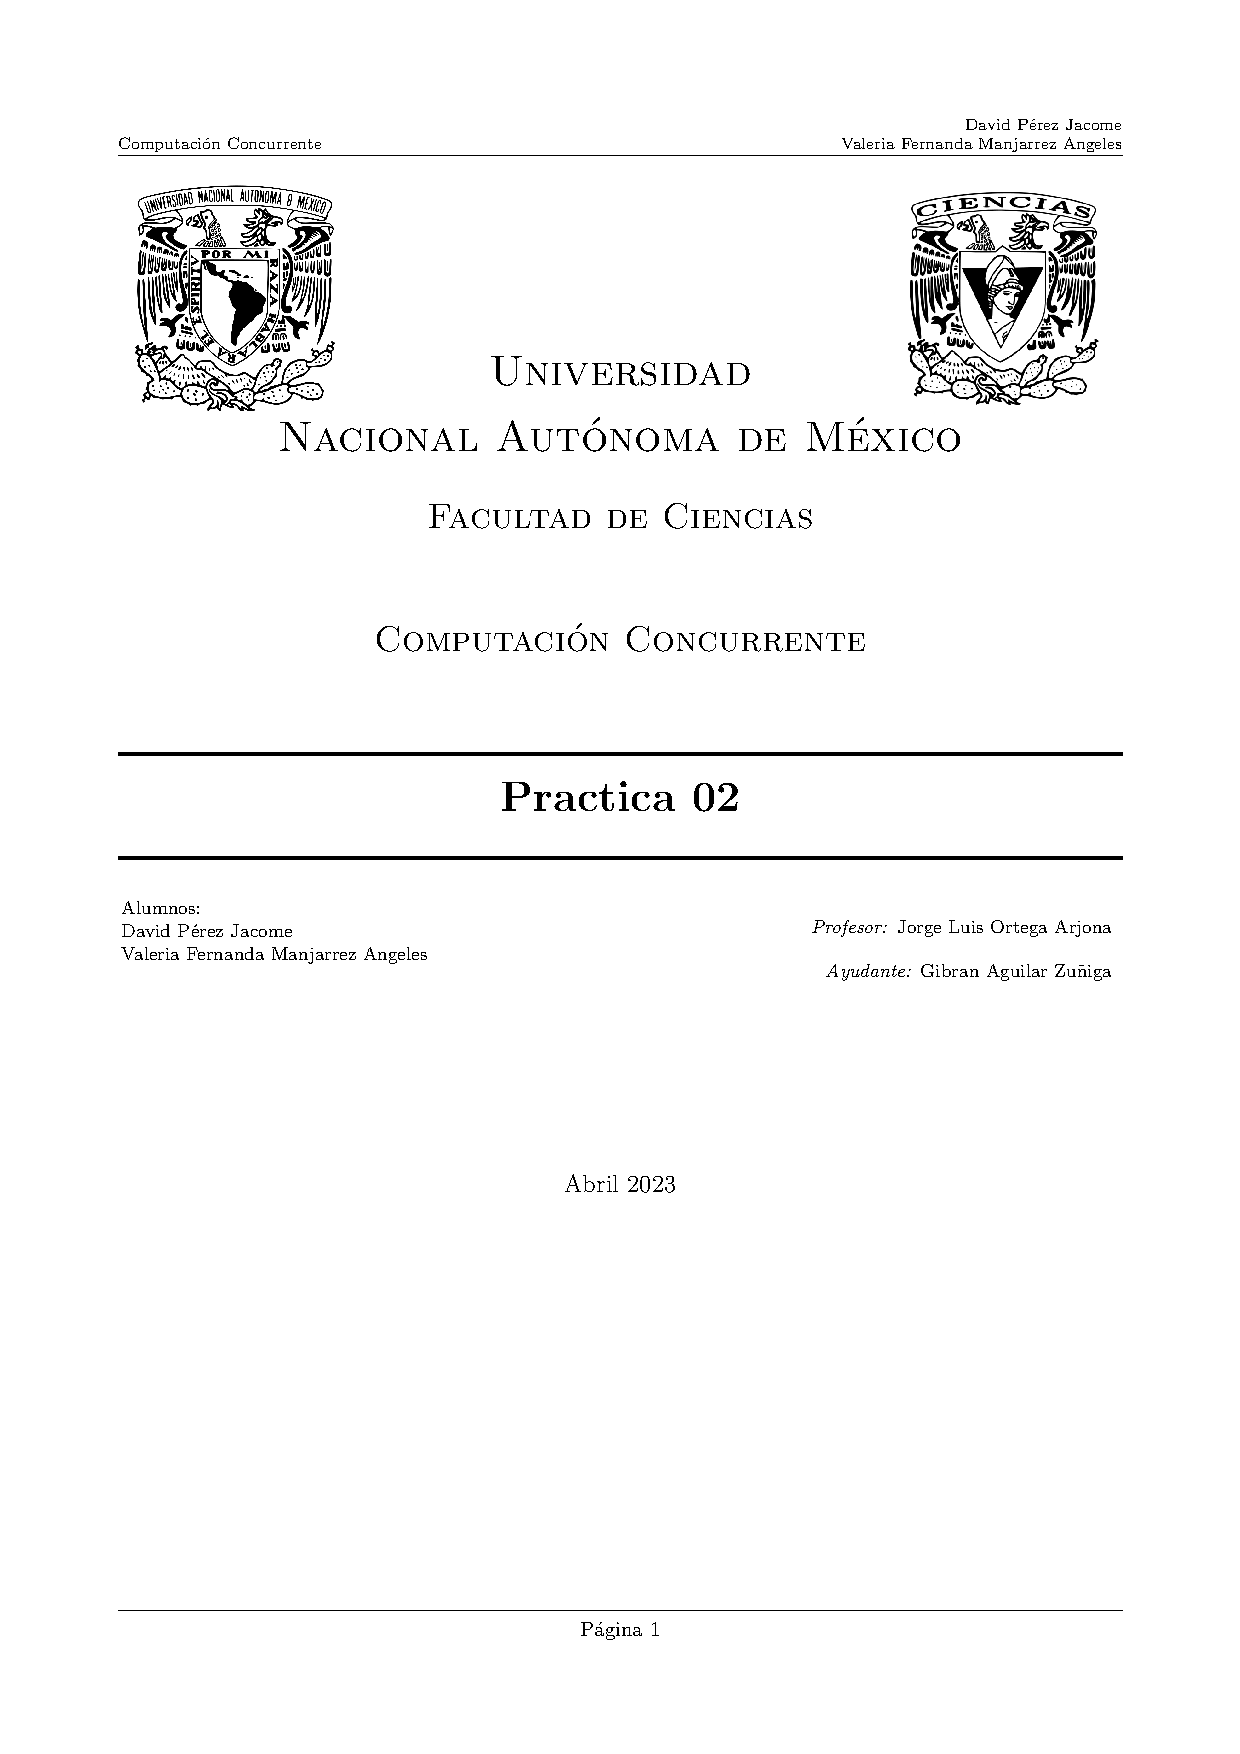
\includepdf{Portada.pdf}
{\color{red} \section*{\textbf{PRACTICA 02}}}
\vspace{1em}

{\color{blue} \subsection*{\textbf{Preguntas:}}}


Deberán detallar a profundidad las respuestas y en caso de ser necesario hacer diagramas 
para ejemplificar tu respuesta.\\


\begin{enumerate}
    \item ¿Qué es un proceso? (1 punto).
    \vspace{2mm}
    
    \textbf{Es el cambio en el estado de la memoria por acción del procesador.}
    \item ¿Qué es la sección crítica de un  proceso? (1 punto).
    \vspace{2mm}
    
    \textbf{Parte del codigo donde se encuentran y modifican los recursos compartidos.}
    \item ¿Qué es el problema libre de hambruna (2 puntos).
    \vspace{2mm}
    
    \textbf{Se refiere a que tenemos que garantizar que los procesos no se queden sin uso de procesador o de recursos que necesite.}
    \item ¿Qué es el problema de abrazos mortales? (2 puntos).
    \vspace{2mm}
    
    \textbf{Es un problema matematico que implica el número de formas en la que se pueden dar la mano varias personas en una reunión sin que existan dos
    aprentones de manos al mismo tiempo. La solución al problema es que el número total de apretones de manos será igual a $\frac{(n(n-1))}{2}$. Esto se debe a que 
    cada persona puede dar la mano a $n-1$ personas diferentes (ya que no puede darse la mano consigo misma), lo que significa que el número total de apretones de manos 
    es igual a la suma de todos los apretones de manos individuales, que es igual a $n(n-1)$. Como cada apretón de manos se cuenta dos veces (una vez por cada persona que la realiza), 
    se divide el resultado por $2$ para obtener el número total de apretones de manos únicos.}
    \item Haz un TDA de Hilos y  un TDA de Semáforos (4 puntos).
    \vspace{2mm}
    
    \textbf{Para semaforos:}\\
    \begin{verbatim}
        / Declaración del TDA de semáforos
TDA_Semaforo:

    // Atributos
    valor: entero
    cola_espera: cola de procesos

    // Métodos wait() y signal()
    crear(valor_inicial: entero) -> semáforo:
        semáforo = nueva instancia de TDA_Semaforo
        semáforo.valor = valor_inicial
        semáforo.cola_espera = nueva cola vacía
        retornar semáforo

    wait(semáforo: semáforo):
        semáforo.valor = semáforo.valor - 1
        si semáforo.valor < 0 entonces:
            agregar proceso actual a cola_espera
            suspender proceso actual

    signal(semáforo: semáforo):
        semáforo.valor = semáforo.valor + 1
        si semáforo.valor <= 0 entonces:
            sacar proceso de cola_espera
            despertar proceso
    \end{verbatim}\\

    \textbf{Para Hilos:}\\
    \begin{verbatim}
        // Declaración del TDA de hilos
TDA_Hilo:

    // Atributos
    id: entero
    estado: enum {ejecutando, listo, bloqueado}
    contexto: contexto del hilo

    // Métodos
    crear(funcion: funcion, argumentos: lista) -> hilo:
        hilo = nueva instancia de TDA_Hilo
        hilo.id = generar_id_unico()
        hilo.estado = listo
        hilo.contexto = crear_contexto(funcion, argumentos)
        retornar hilo

    correr(hilo: hilo):
        cambiar_estado(hilo, ejecutando)
        guardar_contexto(hilo.contexto)
        llamar_funcion(hilo.contexto.funcion, hilo.contexto.argumentos)
        cambiar_estado(hilo, terminado)

    cambiar_estado(hilo: hilo, nuevo_estado: enum):
        hilo.estado = nuevo_estado
    \end{verbatim}
\end{enumerate}

{\color{blue} \subsection*{\textbf{Ejecución:}}}

Para ejecutar nuestro programa es necesario:\\

\begin{enumerate}
    \item Localizarnos en en directorio: \textbf{Practica02}.
    \item Ejecutamos: \textbf{mvn compile}
    \item Ejecutamos el ejecutable que se localiza en el directorio target: \textbf{java -jar target/Practica01.jar}. 
\end{enumerate}
\end{document}